 
 The input values for the question are given in the table \eqref{table:table1}
\begin{table}[ht!]
\centering
\input{./solutions/1/tables/circle/inp.tex}
\caption{Input Values}
\label{table:table1}	
\end{table}
The $\vec{A}$ is at the end of diameter, so the centre$\brak{\vec{O}}$ is the midpoint of $\vec{AB}$.
\begin{align}
\vec{O}=\frac{\vec{A}+\vec{B}}{2}
\\
\vec{A}=2\vec{O}-\vec{B}
\\
\therefore \vec{A}=\myvec{3\\-10}
\end{align}
The python code for the figure \eqref{fig:4.2.1_circle} is\begin{lstlisting}
solutions/1/codes/circle/circle.py
\end{lstlisting}
\begin{figure}[!ht]
\centering
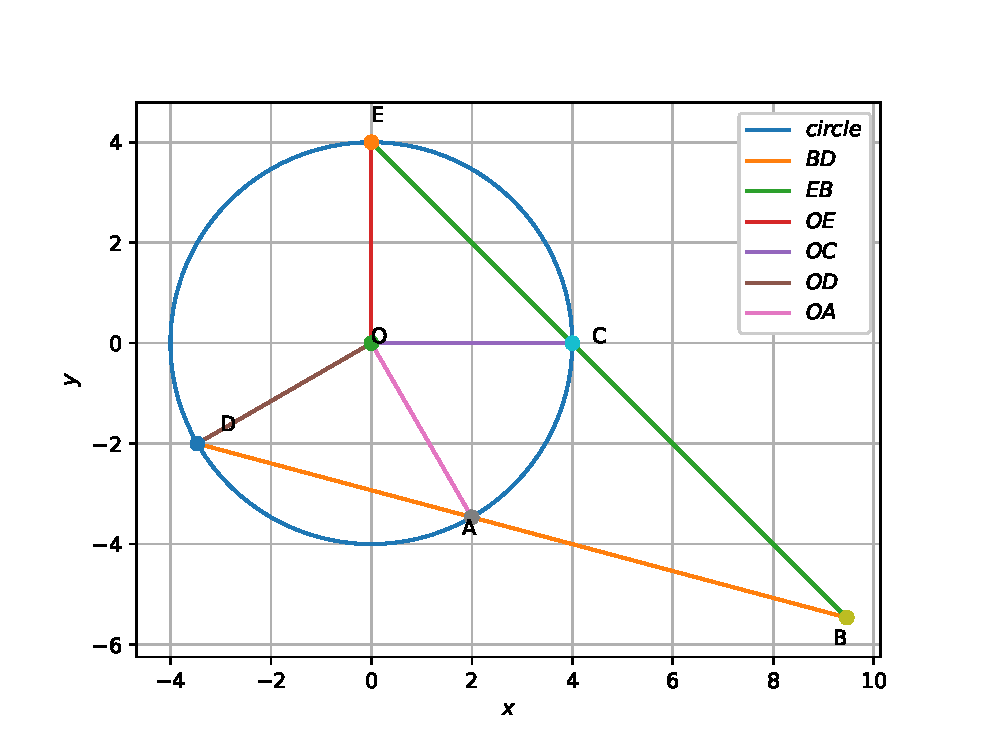
\includegraphics[width=\columnwidth]{./solutions/1/figs/circle/circle.eps}
\caption{}
\label{fig:4.2.1_circle}
\end{figure}

